\documentclass[]{uc2pfecaneva}


\begin{document}
    \setlength{\parskip}{6pt}
    \tableofcontents
    \listoffigures
    \listoftables
    \chapter{Conception}
    \newpage

    \raggedright\section{Introduction}
    \raggedright\section{Domain Model}
    \subsection{Entities}
    \textbf{User :} the super class for all users, contains fields and methods that every user should have.\linebreak
    \textbf{Admin :} the admin user entity, contains admin-specific fields and methods.\linebreak
    \textbf{Teacher :} the super class for all teacher types : Headteacher, TpTdTeacher and Proctor.\linebreak
    \textbf{Headteacher :} the Headteacher user entity.\linebreak
    \textbf{TpTdTeacher :} the TpTdTeacher user entity.\linebreak
    \textbf{Proctor :} the Proctor user entity.\linebreak
    \textbf{Student :} the Student user entity.\linebreak
    \textbf{Exam :} the Exam entity, contains a question list and more.\linebreak
    \textbf{ExamPlanning :} the ExamPlanning entity, contains fields about the starting date of the exam and more.\linebreak
    \textbf{Question :} contains the content of the question.\linebreak
    \textbf{QuestionBank :} contains the question list created the teachers.\linebreak
    \textbf{Module :} the module entity, contains module-specific fields.\linebreak
    \textbf{Report :} contains the report information when a teacher reports a student.\linebreak
    \textbf{Claim :} contains the claim information when a student submits a claim about an evaluation.\linebreak
    \textbf{Response :} the student response of a question.\linebreak
    \textbf{Evaluation :} the response evaluation of a question.\linebreak
    \textbf{Comment :} a comment of a proctor on a student in an exam session\linebreak
    \textbf{Message :} a message between a proctor and a student in an exam session.\linebreak
    \textbf{Absence :} the absence state and information of a student for an exam session.\linebreak
    \textbf{Reminder :} contains a notification content for any user.\linebreak
    \textbf{Answer :} contains the exam answer of an exam, made by the teacher.\linebreak
    \textbf{Feedback :} the student feedback and impression after an exam session.



    \begin{figure}
        \subsection{Domain class diagram}
        \raggedright Defines the domain classes and specifies the relations between these classes
        \linebreak
        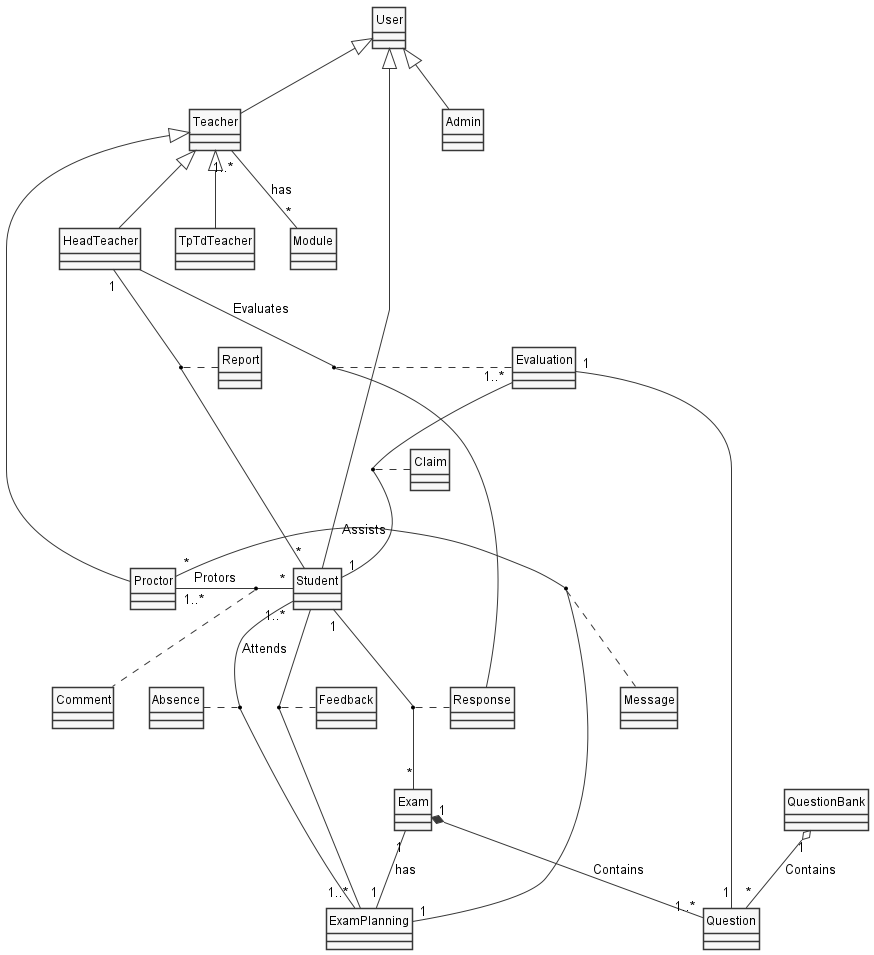
\includegraphics[width=\textwidth]{images/DCD}
        \caption{Domain class diagram}
    \end{figure}




    \begin{figure}
        \subsection{Conception class diagram}
        \raggedright Defines the conceptual classes with details, specifying the fields and methods of each class.
        \linebreak
        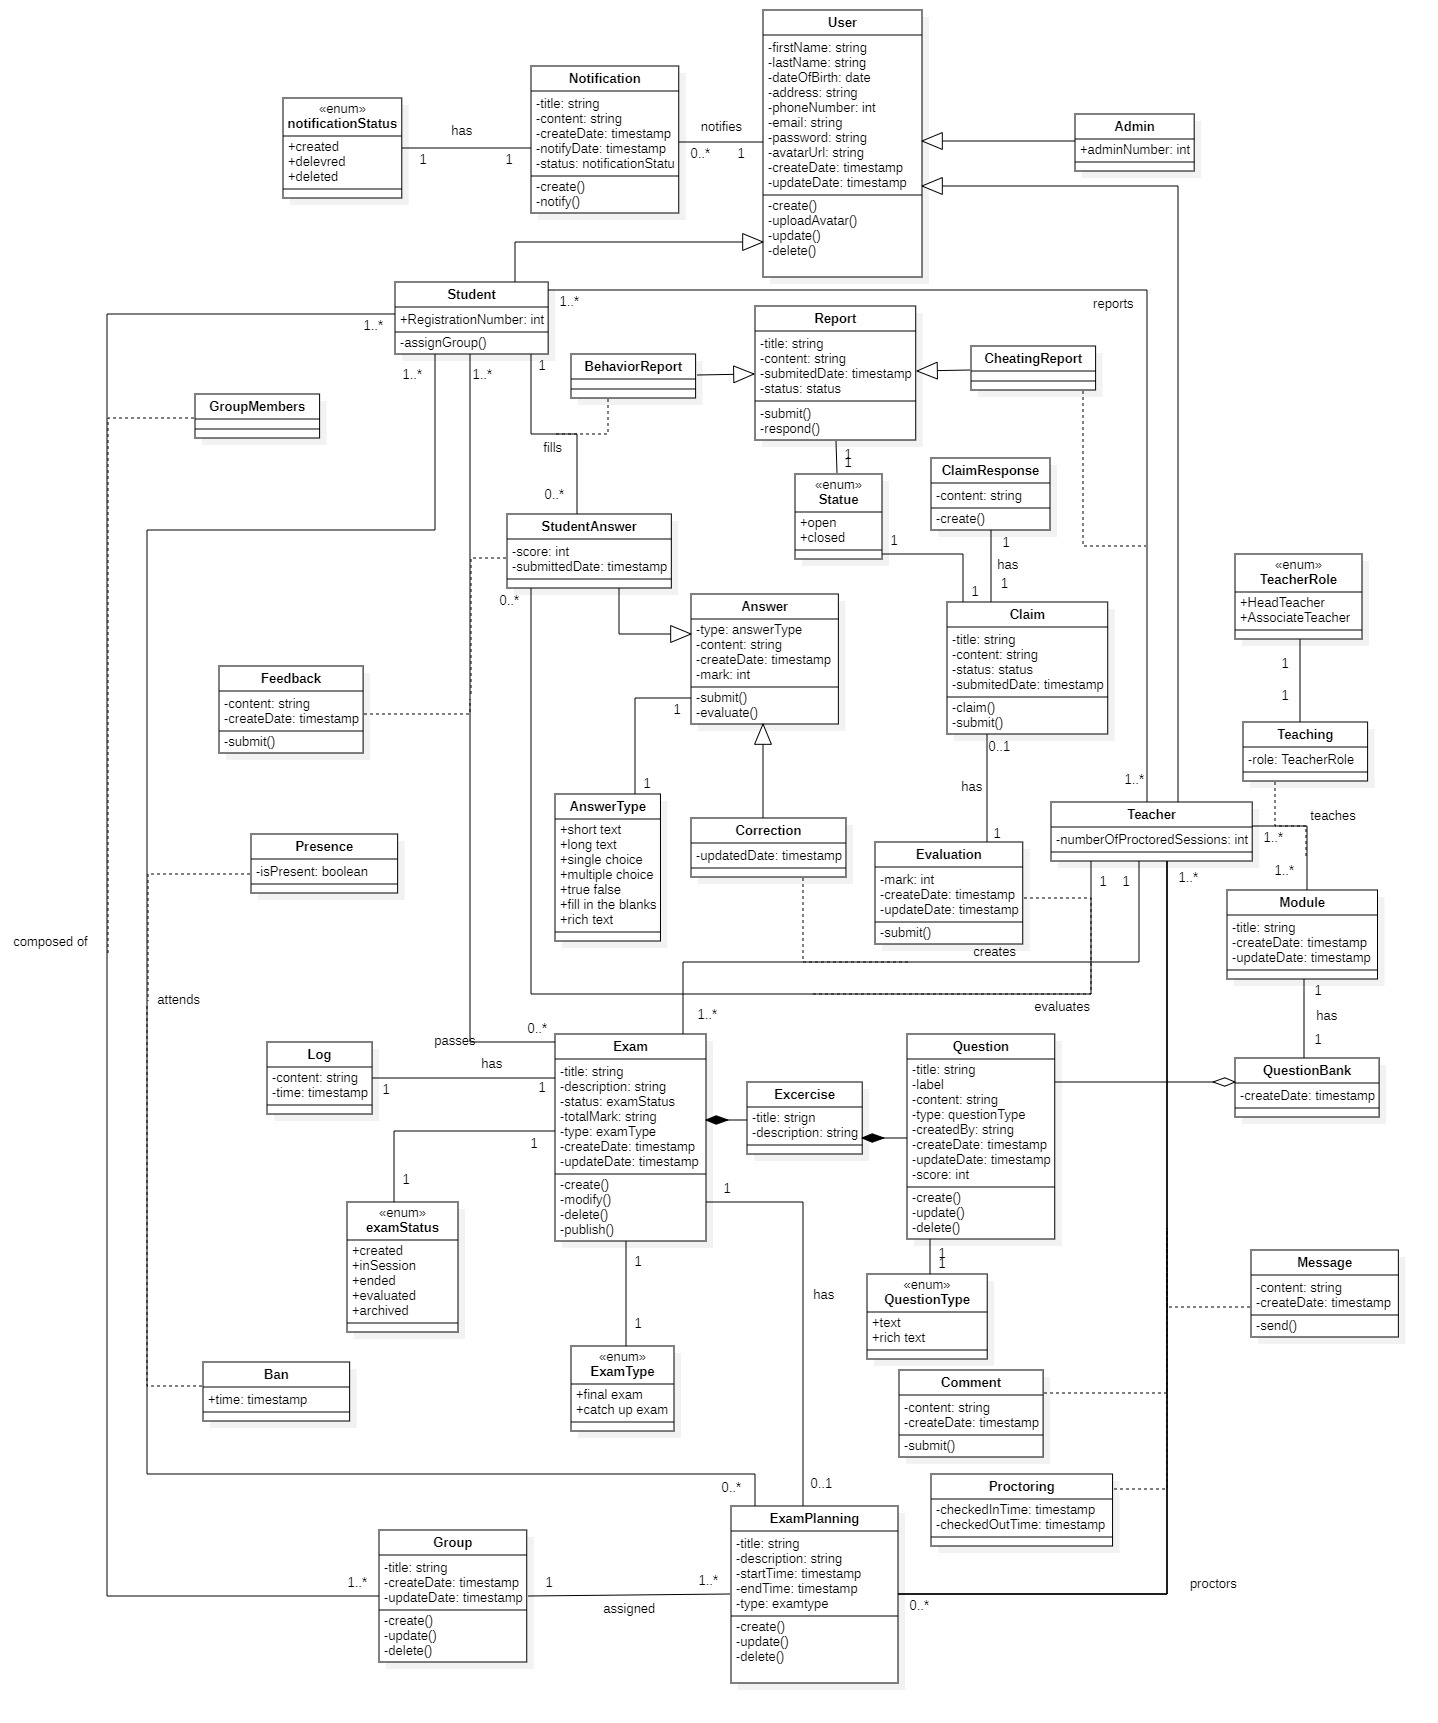
\includegraphics[width=350pt]{images/CCD}
        \caption{Conception class diagram}
    \end{figure}
    \clearpage

    \raggedright\section{Migration to a database}
    \raggedright\section{Conclusion}


\end{document}